\documentclass{jsarticle}
 
\usepackage[dvipdfmx]{graphicx}
\usepackage{tikz}
 
\begin{document}
 
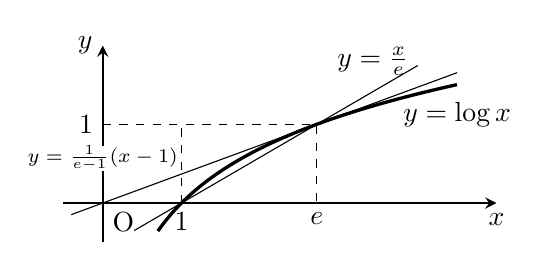
\begin{tikzpicture}
 
   % 座標軸
   \draw [thick, -stealth](-0.5,0)--(5,0) node [anchor=north]{$x$};
   \draw [thick, -stealth](0,-0.5)--(0,2) node [anchor=east]{$y$};
   \node [anchor=north west] at (0,0) {O};
 
   % y=log(x)
   \draw [very thick, domain=0.7:4.5, samples=200] plot(\x, {ln(\x)});
   \node [anchor=north] at (4.5,1.4){$y=\log x$};
 
   % y=x/e
   \draw [domain=-0.4:4.5] plot(\x,\x/e);
   \node [anchor=east] at(4,1.8){$y=\frac{x}{e}$};
 
   % y=(x-1)/(e-1)
   \draw [domain=0.4:4] plot(\x, {(\x-1)/(e-1)});
   \node [anchor=south, font=\scriptsize, fill=white, inner sep=0pt] at(0,0.4){$y=\frac{1}{e-1}(x-1)$};
 
   % 補助線
   \draw [dashed](0,1) node [anchor=east]{$1$}--(e,1)--(e,0) node[anchor=north]{$e$};
   \draw [dashed](1,0) node [anchor=north]{$1$}--(1,1);
 
\end{tikzpicture}
\vspace{20mm} \\
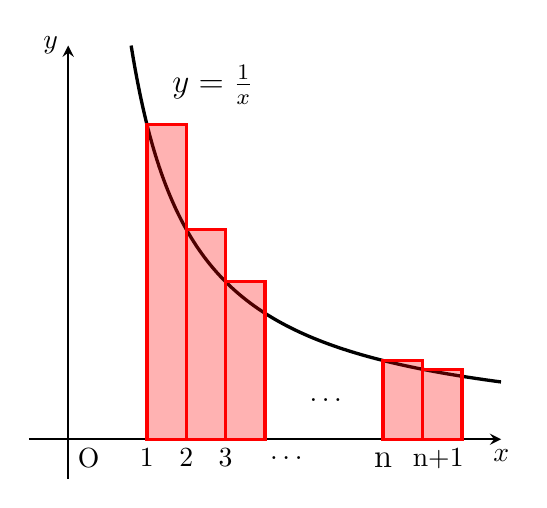
\begin{tikzpicture}
  
  % 座標軸
  \draw [thick, -stealth](-0.5,0)--(5.5,0) node [anchor=north]{$x$};
  \draw [thick, -stealth](0,-0.5)--(0,5) node [anchor=east]{$y$};
  \node [anchor=north west] at (0,0) {O};
  
  % y=1/x
  \draw [very thick, domain=0.8:5.5, samples=200] plot(\x, 4/\x);
  \node [anchor=west] at (1.2,4.5) {\large $y=\frac{1}{x}$};
  
  % 長方形(k=1)
  \draw [very thick, draw=red] (1,0) rectangle (1.5,4);
  \fill [red, opacity=.3] (1,0) rectangle (1.5,4);
  \node [anchor=north] at (1,0) {1};
  
  % 長方形(k=2)
  \draw [very thick, draw=red] (1.5,0) rectangle (2,4/1.5);
  \fill [red, opacity=.3] (1.5,0) rectangle (2,4/1.5);
  \node [anchor=north] at (1.5,0) {2};
  
  % 長方形(k=3)
  \draw [very thick, draw=red] (2,0) rectangle (2.5,2);
  \fill [red, opacity=.3] (2,0) rectangle (2.5,2);
  \node [anchor=north] at (2,0) {3};
  
  % 長方形(k=n)
  \draw [very thick, draw=red] (4,0) rectangle (4.5,1);
  \fill [red, opacity=.3] (4,0) rectangle (4.5,1);
  \node [anchor=north] at (4,-0.05) {\large n};
  
  % 長方形(k=n+1)
  \draw [very thick, draw=red] (4.5,0) rectangle (5,4/4.5);
  \fill [red, opacity=.3] (4.5,0) rectangle (5,4/4.5);
  \node [anchor=north] at (4.7,0) {n+1};
  
  % …の挿入
  \node at (3.3,0.5) {\ldots};
  \node [anchor=north] at (2.8,-0.1) {\ldots};
  
\end{tikzpicture}

 
\end{document}